\section{Design}
\subsection{Architettura}

In fase di progettazione abbiamo scelto di adottare il pattern architetturale MVC, traendone quindi tutti i suoi vantaggi, principalmente che model e controller rimangono praticamente uguali a prescindere dalla view utilizzata. Infatti, abbiamo scelto nella view di usare il pattern Strategy e applicare il principio del "Composition over inheritance", definendo quindi delle interfacce generiche per i singoli componenti che potranno perciò adottare qualsiasi GUI framework. Per passare, per esempio da Swing a JavaFX basterebbe solo sostituire le implementazioni delle interfacce presenti nella parte di view. Ogni modulo del pattern Model-View-Controller ha quindi una propria organizzazione e scopo:
\begin{itemize}
    \item Model, (parlare del Mediator che gestisce la doppia referenza e del Mutable/non Mutable, insieme a Factory, Builder e Strategy)
    \item View, (parlare del fatto che la UserInterface è l'interfaccia principale che pilota tutto, del Composition over inheritance e delle matrioska di Component/JPanel nella quale vengono diffusi aggiornamenti (update) ed informazioni)
    \item Controller, (parlare di come gestisce la partita e di come si occupa della lettura della configurazione (ConfigurationLoader))
\end{itemize}
Siccome ad ogni modifica di stato della partita, il Controller notifica le UserInterface collegate ad esso, possiamo giocare alla stessa partita contemporaneamente tramite varie interfacce utente aggiungendole tutte allo stesso controller. Queste possono essere diverse tra loro e di qualsiasi tipo, per esempio: Web, CLI o come nel nostro caso, GUI.

\subsection{Design dettagliato}

\subsection*{Mauro Pellonara}

\subsection*{Alessandro Martini}
\subsubsection*{Definizione di operazioni che vengono utilizzati su GameSet differenti}
\begin{figure}[ht]
    \centering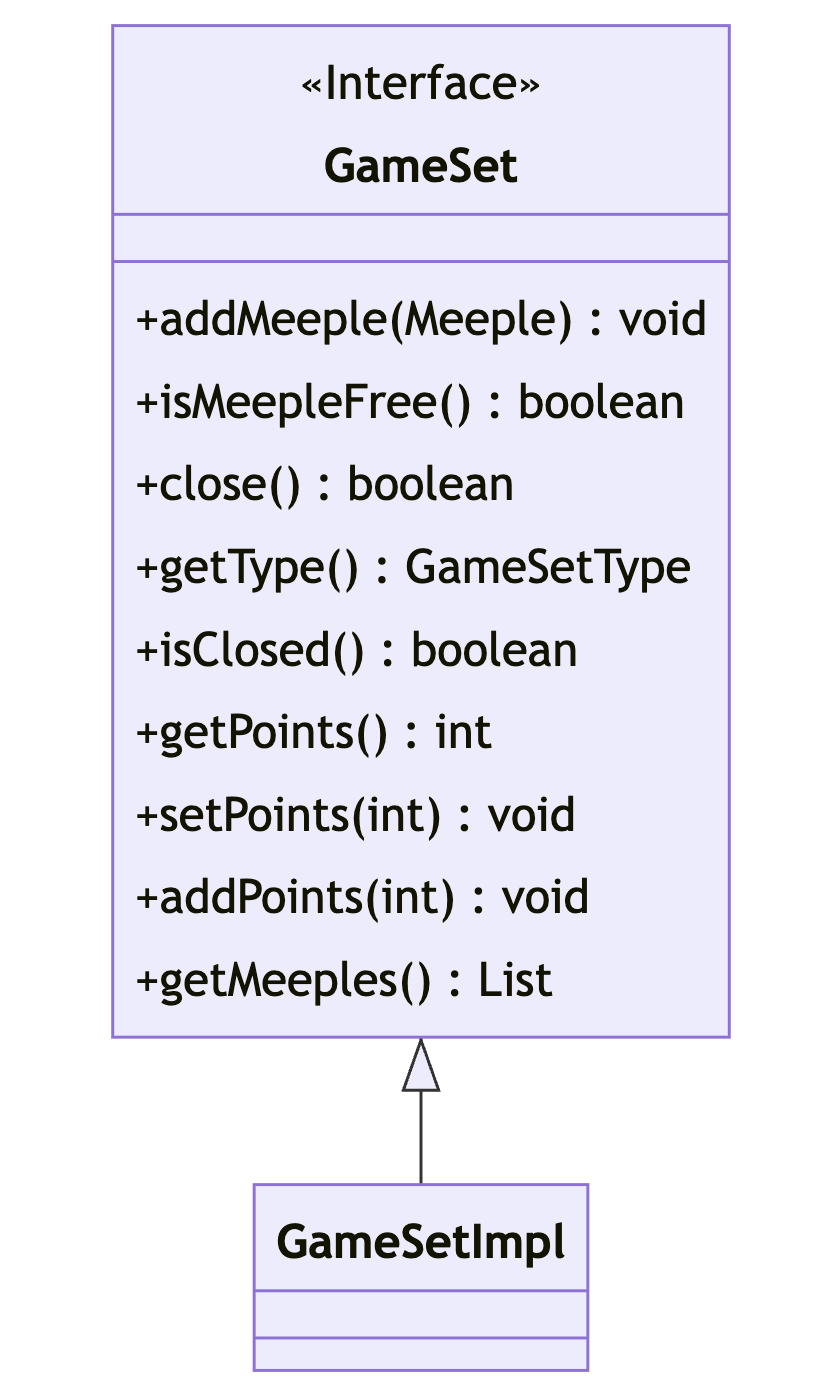
\includegraphics[scale=.4]{images/gameset.png}
    \caption{Rappresentazione UML dell'applicazione del pattern Strategy per il GameSet e GameSetImpl}
\end{figure}
\paragraph{Problema:}
A ogni GameSet, va assegnato il relativo punteggio, il controllo se vi sono meeple presenti e la possibilità di piazzarli, la tipologia del GameSet e infine se è ancora aperto o chiuso.
\paragraph{Soluzione:}
La classe GameSetImpl implementa lo Strategy pattern, avendo come riferimento GameSet che serve come strategy per la gestione delle informazioni di ogni singolo GameSet.

\subsubsection*{Creazione di più GameSet con tipologie differenti}
\begin{figure}[ht]
    \centering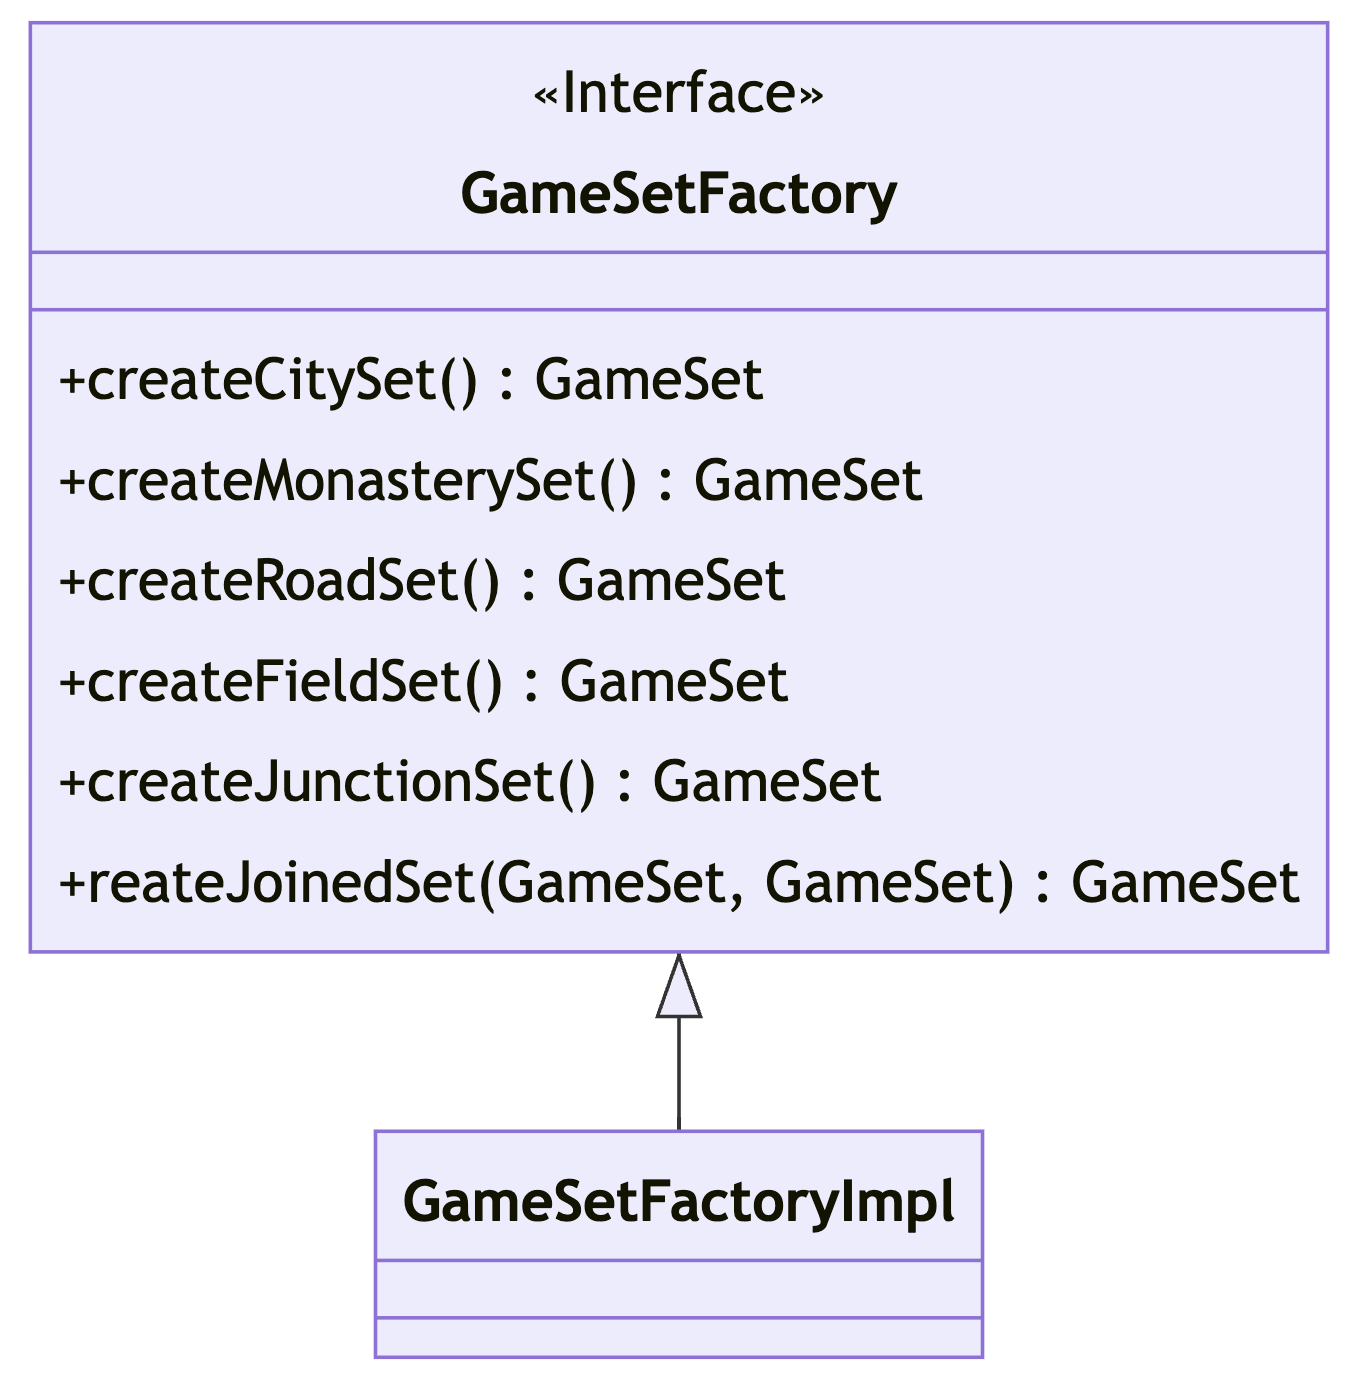
\includegraphics[scale=.3]{images/gamesetfactory.png}
    \caption{Rappresentazione UML dell'applicazione del pattern Strategy per il gamesetfactory e GameSetFactoryImpl}
\end{figure}

\paragraph{Problema:}
Possono esistere più GameSet con informazioni differenti e relativi punteggi assegnati, in aggiunta si devono gestire l'unione di due GameSet.
\paragraph{Soluzione:}
La classe GameSetFactoryImpl implementa lo Strategy pattern, avendo come riferimento GameSetFactory che serve come strategy per la creazione di nuovi GameSet.

\subsection*{Davide Speziali}

\subsection*{Samuele Giancarli}
